\begin{enumerate}
\item In a given $8$-bit general purpose micro-controller there are following flags. $C$-Carry, $A$-Auxiliary Carry, $O$-Overflow flag, $P$-Parity ($0$ for even, $1$ for odd) $R0$ and $R1$ are the two general purpose registers of the micro-controller.After execution of the following instructions, the decimal equivalent of the binary sequence of the flag pattern $[CAOP]$ will be $\underline{\hspace{1cm}}$.\\


\begin{lstlisting}
MOV R0,+0x60
MOV R1,+0x46 
ADD R0,R1
\end{lstlisting}
    
\hfill{(EE GATE 2023)}\\


\item 
Consider the given C-code and its corresponding assembly code, with a few operands U1-U4 being unknown. Some useful information as well as the semantics of each unique assembly instruction is annotated as inline comments in the code.  

\begin{figure}[H]
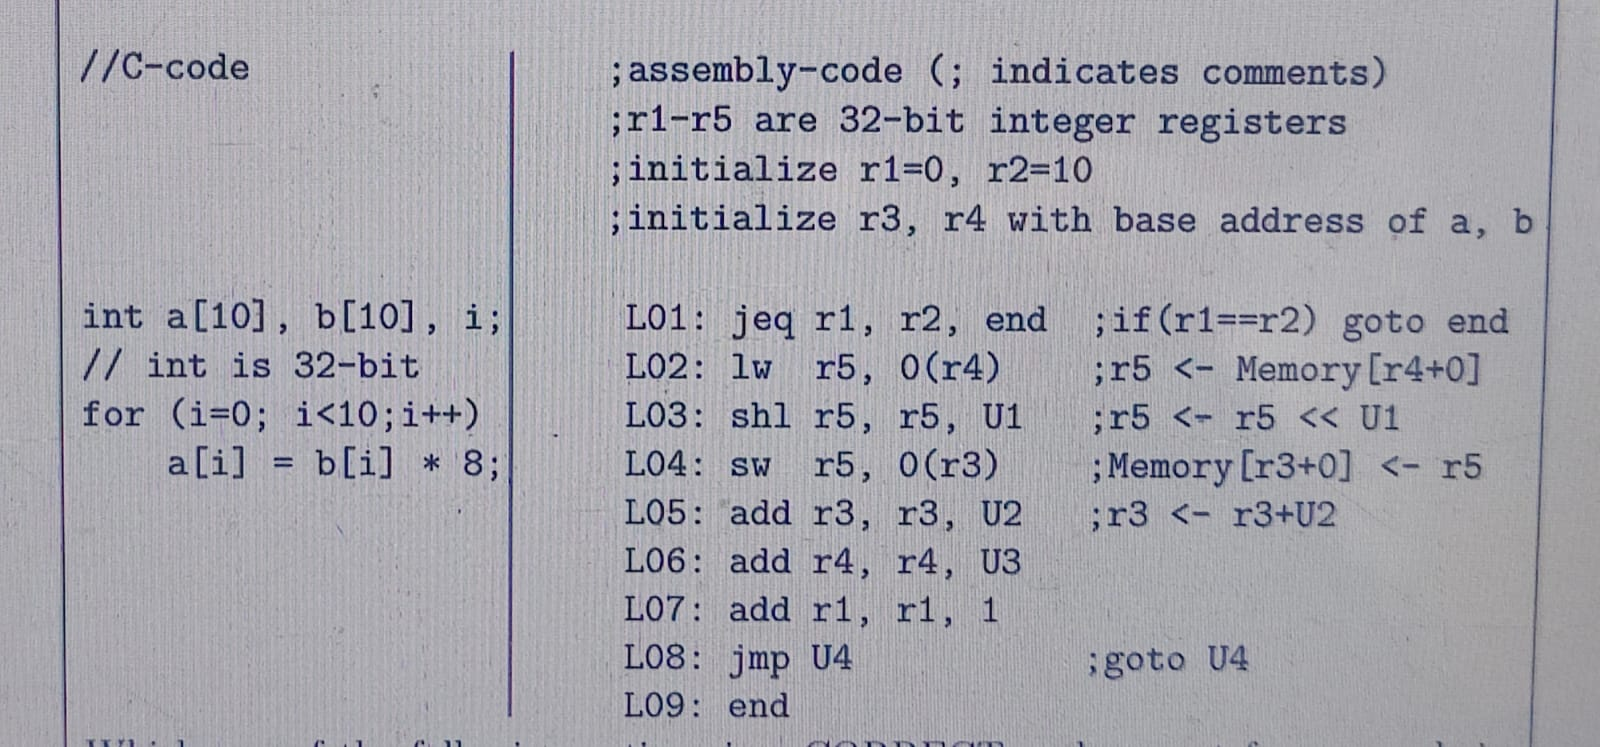
\includegraphics[width=\columnwidth]{figs/cse.jpeg} 
\caption{code}                                       
\label{fig:code}
\end{figure}

\item Which one of the following options is a CORRECT replacement 
for operands in the position (U1,U2,U3,U4) in the above 
assembly code?

\begin{enumerate}
\item (8,4,1,L02)                      
\item (3,4,4,L01)
\item (8,1,1,L02)                             
\item (3,1,1,L01)         
\end{enumerate}

\end{enumerate}
